%%
% The BIThesis Template for Bachelor Paper Translation
%
% 北京理工大学毕业设计(论文) —— 使用 XeLaTeX 编译
%
% Copyright 2020-2023 BITNP
%
% This work may be distributed and/or modified under the
% conditions of the LaTeX Project Public License, either version 1.3
% of this license or (at your option) any later version.
% The latest version of this license is in
%   http://www.latex-project.org/lppl.txt
% and version 1.3 or later is part of all distributions of LaTeX
% version 2005/12/01 or later.
%
% This work has the LPPL maintenance status `maintained'.
%
% The Current Maintainer of this work is Feng Kaiyu.
%
% Compile with: xelatex -> biber -> xelatex -> xelatex
%%

% 第一章节

\chapter{引言}

三维点云配准\cite{TEASER, DCP, paulj1992method}主要关注在源点云和目标点云之间估计一个单一的变换。然而,我们有时可能希望在点云之间估计多个变换。例如,我们有一个物体的3D扫描,可能希望在目标点云中找到如图\ref{fig:problem}所示的同一物体在桌子上的姿态。这个问题,我们称之为多实例点云配准,文献中较少研究。这个问题,我们称之为多实例点云配准,文献中较少研究。将现有的点云配准方法扩展到解决这个问题并非易事。

主要的挑战是在嘈杂的对应关系集合中识别属于不同实例的对应点的不同簇。一种解决方案是采用3D物体检测器或将实例分割应用于目标点云。然后,通过常规的点云配准方法估计每个实例的姿态。然而,这种方法需要为特定对象或类别训练检测器或分割网络\cite{VoteNet, Occuseg},不适用于未知对象或任意3D扫描。

\begin{figure}[htbp]
  \centering
  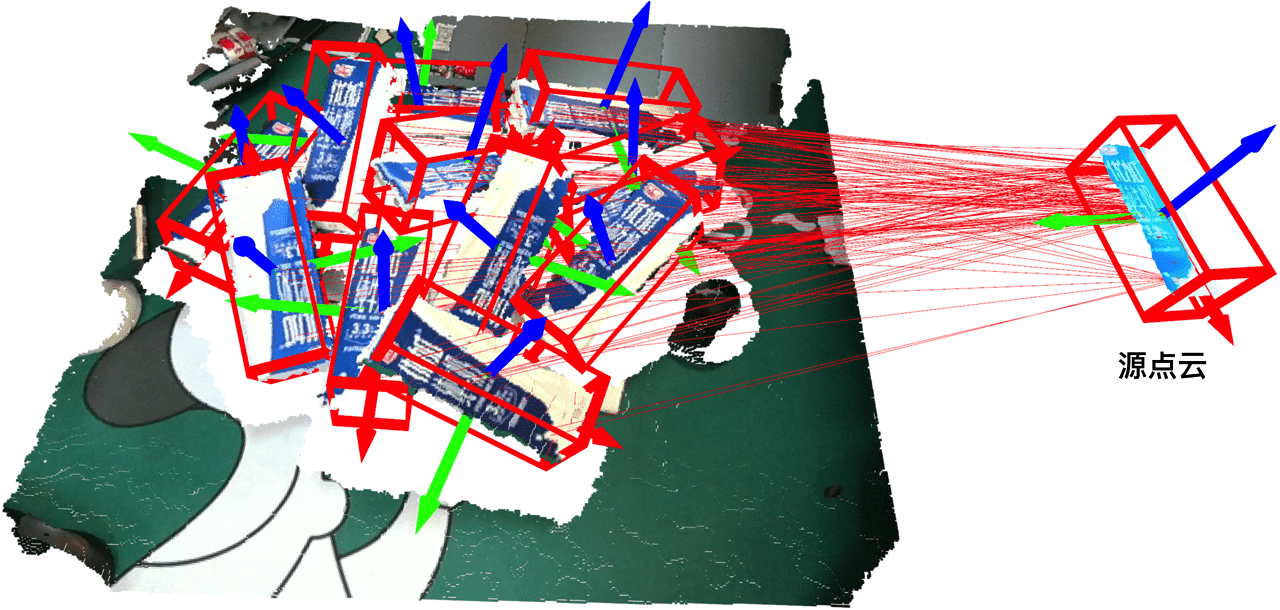
\includegraphics[width=0.8\textwidth]{images/problem.png}
  \caption{多实例点云配准:给定一个物体的源点云,多实例配准需要估计目标点云中每个物体的姿态。}
  \label{fig:problem} % label 用来在文中索引
  \vspace{-0.5in}
\end{figure}



另一种解决方案是通过多模型拟合\cite{Tlinkage, RPA, Coverage}或\cite{MCT, CONSAC, ProgressiveX2}。现有的多模型拟合方法依赖于采样有效的假设,当模型数量或异常值比例变高时,涉及大量的采样步骤,使得这些算法的效率和鲁棒性急剧下降。

在本文中,我们提出了一种鲁棒且高效的多实例三维配准问题解决方案。关键思想是根据距离不变性矩阵直接将对应点分组到不同的簇中。具体而言,在使用诸如D3Feat \cite{D3Feat}、PREDATOR \cite{PREDATOR}或SIFT \cite{lowe2004distinctive}等描述符进行特征匹配得到点对应关系之后,通过检查每对对应关系之间的距离一致性来构造矩阵。我们发现这个矩阵的行或列向量具有强大的表示能力,可以用于识别特定实例的对应关系集合。因此,我们应用了一种简单且高效的聚类算法将这些对应关系划分为团。通过将相似簇合并并重新分配簇id给每个对应关系,递归地进行几步细化聚类。最后,通过一个简单的排序策略自动识别每个实例的异常值和内点。



由于不需要耗时的假设采样,我们的方法具有很高的效率。我们在合成数据集和真实世界数据集上进行了广泛的实验。结果表明,我们的方法在准确性和鲁棒性方面表现明显优于现有方法,速度至少快10倍。总之,我们的贡献包括:
\begin{itemize}
\setlength{\itemsep}{-1pt}
\setlength{\parsep}{-2pt}
\item 我们提出了一种针对多实例点云配准问题的高效且鲁棒的解决方案,其在准确性、鲁棒性和速度方面都具有优越的性能。
\item 我们提出使用三个指标(平均命中召回率、平均命中精确度和平均命中F1)来全面评估多实例点云配准的性能。%据我们所知,尚未有针对这类评估的指标提出。
\item 我们的解决方案可以用于零样本检测3D物体,正如我们的真实世界测试所示。
\end{itemize}

